\section{Prior work}
In this section we describe our current model for understanding polite speech as reflecting tradeoff between information transfer and face-saving, and the current empirical support for this model. These results have been reported to the Cognitive Science Conference in \citet{yoon2016}. 

\subsection{Current model}

Politeness poses a challenge for formal models of pragmatic language understanding, which assume that speakers' goals are to communicate informatively about some aspect of the world. The Rational Speech Act (RSA) framework \citep{Frank2012, Goodman2013} describes language understanding as recursive probabilistic inference between a pragmatic listener and an informative speaker. This framework has been successful at capturing the quantitative details of a number of language understanding tasks, but it neglects the social goals a speaker may pursue. Our model extends RSA to take into account a speaker with both the usual epistemic goal and a competing social goal: be kind (i.e., save face).

RSA models a listener as reasoning about a speaker, who chooses utterances approximately optimally given a utility function. \citet{Goodman2013} define speaker utility by the amount of information a \emph{literal listener} would still not know about world state $s$ after hearing a speaker's utterance $w$ (i.e. \emph{surprisal}), what we will call \emph{epistemic utility}:
$U_{epistemic}(w; s) = \ln(P_{L_0}(s \mid w)) $,
where the literal listener is a simple Bayesian agent that takes the utterance to be true.

In our new model, ``Polite RSA,'' we propose there is a second component to the speaker's utility related to the intrinsic value of the state in the eyes of the listener, what we will call \emph{social utility}.
We define the social utility of an utterance to be the expected utility of the state the listener would infer given the utterance $w$:
$$
U_{social}(w; s) = \mathbb{E}_{P_{L_0}(s \mid w)}[V(s)],
$$
%
where $V$ is a value function that maps states to subjective utility values---this captures the affective consequences for the listener of being in state $s$.
%
We take the overall speaker utility to be a weighted combination of epistemic and social utilities:
$$
U(w;s;  \hat{\beta}) = \beta_{epistemic}\cdot U_{epistemic} + \beta_{social} \cdot U_{social}.
$$

The speaker chooses utterances $w$ softmax-optimally given the state $s$ and his goal weights $\hat{\beta}$. The pragmatic listener, denoted $L_1$, infers the world state based on this speaker model. We will assume the listener does not know exactly how the speaker weights his competing goals, however.
Following the treatment of RSA using lifted variables \citep{GoodmanLassiter2015, bergen2016, Kao2014},
we assume the pragmatic listener jointly infers the state $s$ and the utility weights of the speaker, $\beta_{epistemic}$ and $\beta_{social}$:
\begin{equation}
P_{L_1}(s,  \hat{\beta} \mid w)\propto P_{S_1}(w \mid s,  \hat{\beta})\cdot P(s) \cdot P( \hat{\beta}) \label{eq:L1}
\end{equation}

We implemented this model using the probabilisitic programming language WebPPL \cite{dippl} and a complete implementation can be found at \url{http://forestdb.org/models/politeness-cogsci2016.html}.


\subsection{Empirical support for the Polite RSA}

The predictions of Polite RSA were tested in two Experiments. Here we provide details on both experiments, as they will be identical in structure to proposed experiments in Section 3.2.3. 
Within our experimental domain, we assume there are five possible states of the world corresponding to the value placed on a particular referent (e.g. the presentation the speaker is commenting on): $S = \{s_{1}, ...,  s_{5}\}$.
We further assume a uniform prior distribution over possible states of the world.
The states have subjective numerical values $V(s_{i}) = \alpha \cdot i$, where $\alpha$ is a scaling parameter (later inferred from data).
The set of utterances is \{\emph{terrible}, \emph{bad}, \emph{okay}, \emph{good}, and \emph{amazing}\}.

\subsubsection{Experiment 1: True state inference}

We examined listeners' inferences about the likely state of the world $s$ given a speaker's utterance (e.g. ``It was good'') and a description of the speaker's intentions (e.g. the speaker wanted to be nice). We presented scenarios in which a person (e.g. Ann) asked for another person (e.g. Bob)'s opinion on her performance. We provided information on Bob's goal (to be \emph{honest}, \emph{nice}, or \emph{mean}) and what Bob actually said to Ann (e.g. ``It [your cake] was okay''), where Bob used one of the five possible words: \emph{terrible}, \emph{bad}, \emph{okay}, \emph{good}, or \emph{amazing}. Then we asked participants to infer the true state of the world (e.g. how Bob actually felt about Ann's cake). Thus, participants read each story (e.g. Ann baked a cake and asked Bob about it) followed by a prompt that said,
e.g., ``Bob wanted to be nice: ``It was okay,'' he said. How do you think Bob actually felt about Ann's cake?''
Participants indicated their answer on a scale of five hearts.\footnote{The experiment can be viewed at: \url{http://langcog.stanford.edu/expts/EJY/polgrice/L2_S/polgrice_L2_S.html.}} 

\subsubsection{Experiment 2: Goal inference}

Experiment 2 probed listeners' inferences of the speaker's goals, given an utterance (e.g. \emph{``It was good''}) and a true state. We presented the same context items and utterances as Experiment 1. But instead of goals, we provided information on the true states (i.e. how Bob actually felt towards Ann's performance).
Then we asked participants to infer the likelihood of Bob's goals to be \emph{honest}, \emph{nice}, and \emph{mean}.
Participants read each scenario followed by a question that read, ``Based on what Bob said, how likely do you think that Bob's goal was to be: honest; nice; mean,'' with the three goals placed in a random order below three slider bars, on which the participant could indicate each goal's likelihood.\footnote{The experiment can be viewed at: \url{http://langcog.stanford.edu/expts/EJY/polgrice/L2_G/polgrice_L2_G.html.}}

\subsubsection{Findings}

The findings were consistently in favor of the model predictions: participants' inferences about the true state of the world (e.g. how much Ann actually liked the talk that Bob gave) differed based on what the speaker said (e.g. Ann said ``It was okay'') and whether the speaker's intended goal was to be honest, nice or mean. For example, when the speaker wanted to be nice and said ``It was okay,'' participants predicted that Ann actually thought it was mediocre (2 out of 5; see Figure~\ref{fig:expt2}). Also, participants' attributions of different social goals to speakers depended on how well the literal utterance meaning matched the actual rating the performance deserved. When Ann actually thought Bob's talk was bad but said ``It was good'', then people attributed more niceness and less honesty to Ann. Overall, our Polite RSA model displayed strong quantitative fits to the inference data in both experiments ($r^2(75) = 0.74$ and $r^2(75) = 0.82$, respectively).

\begin{figure*}[h]
\begin{centering}
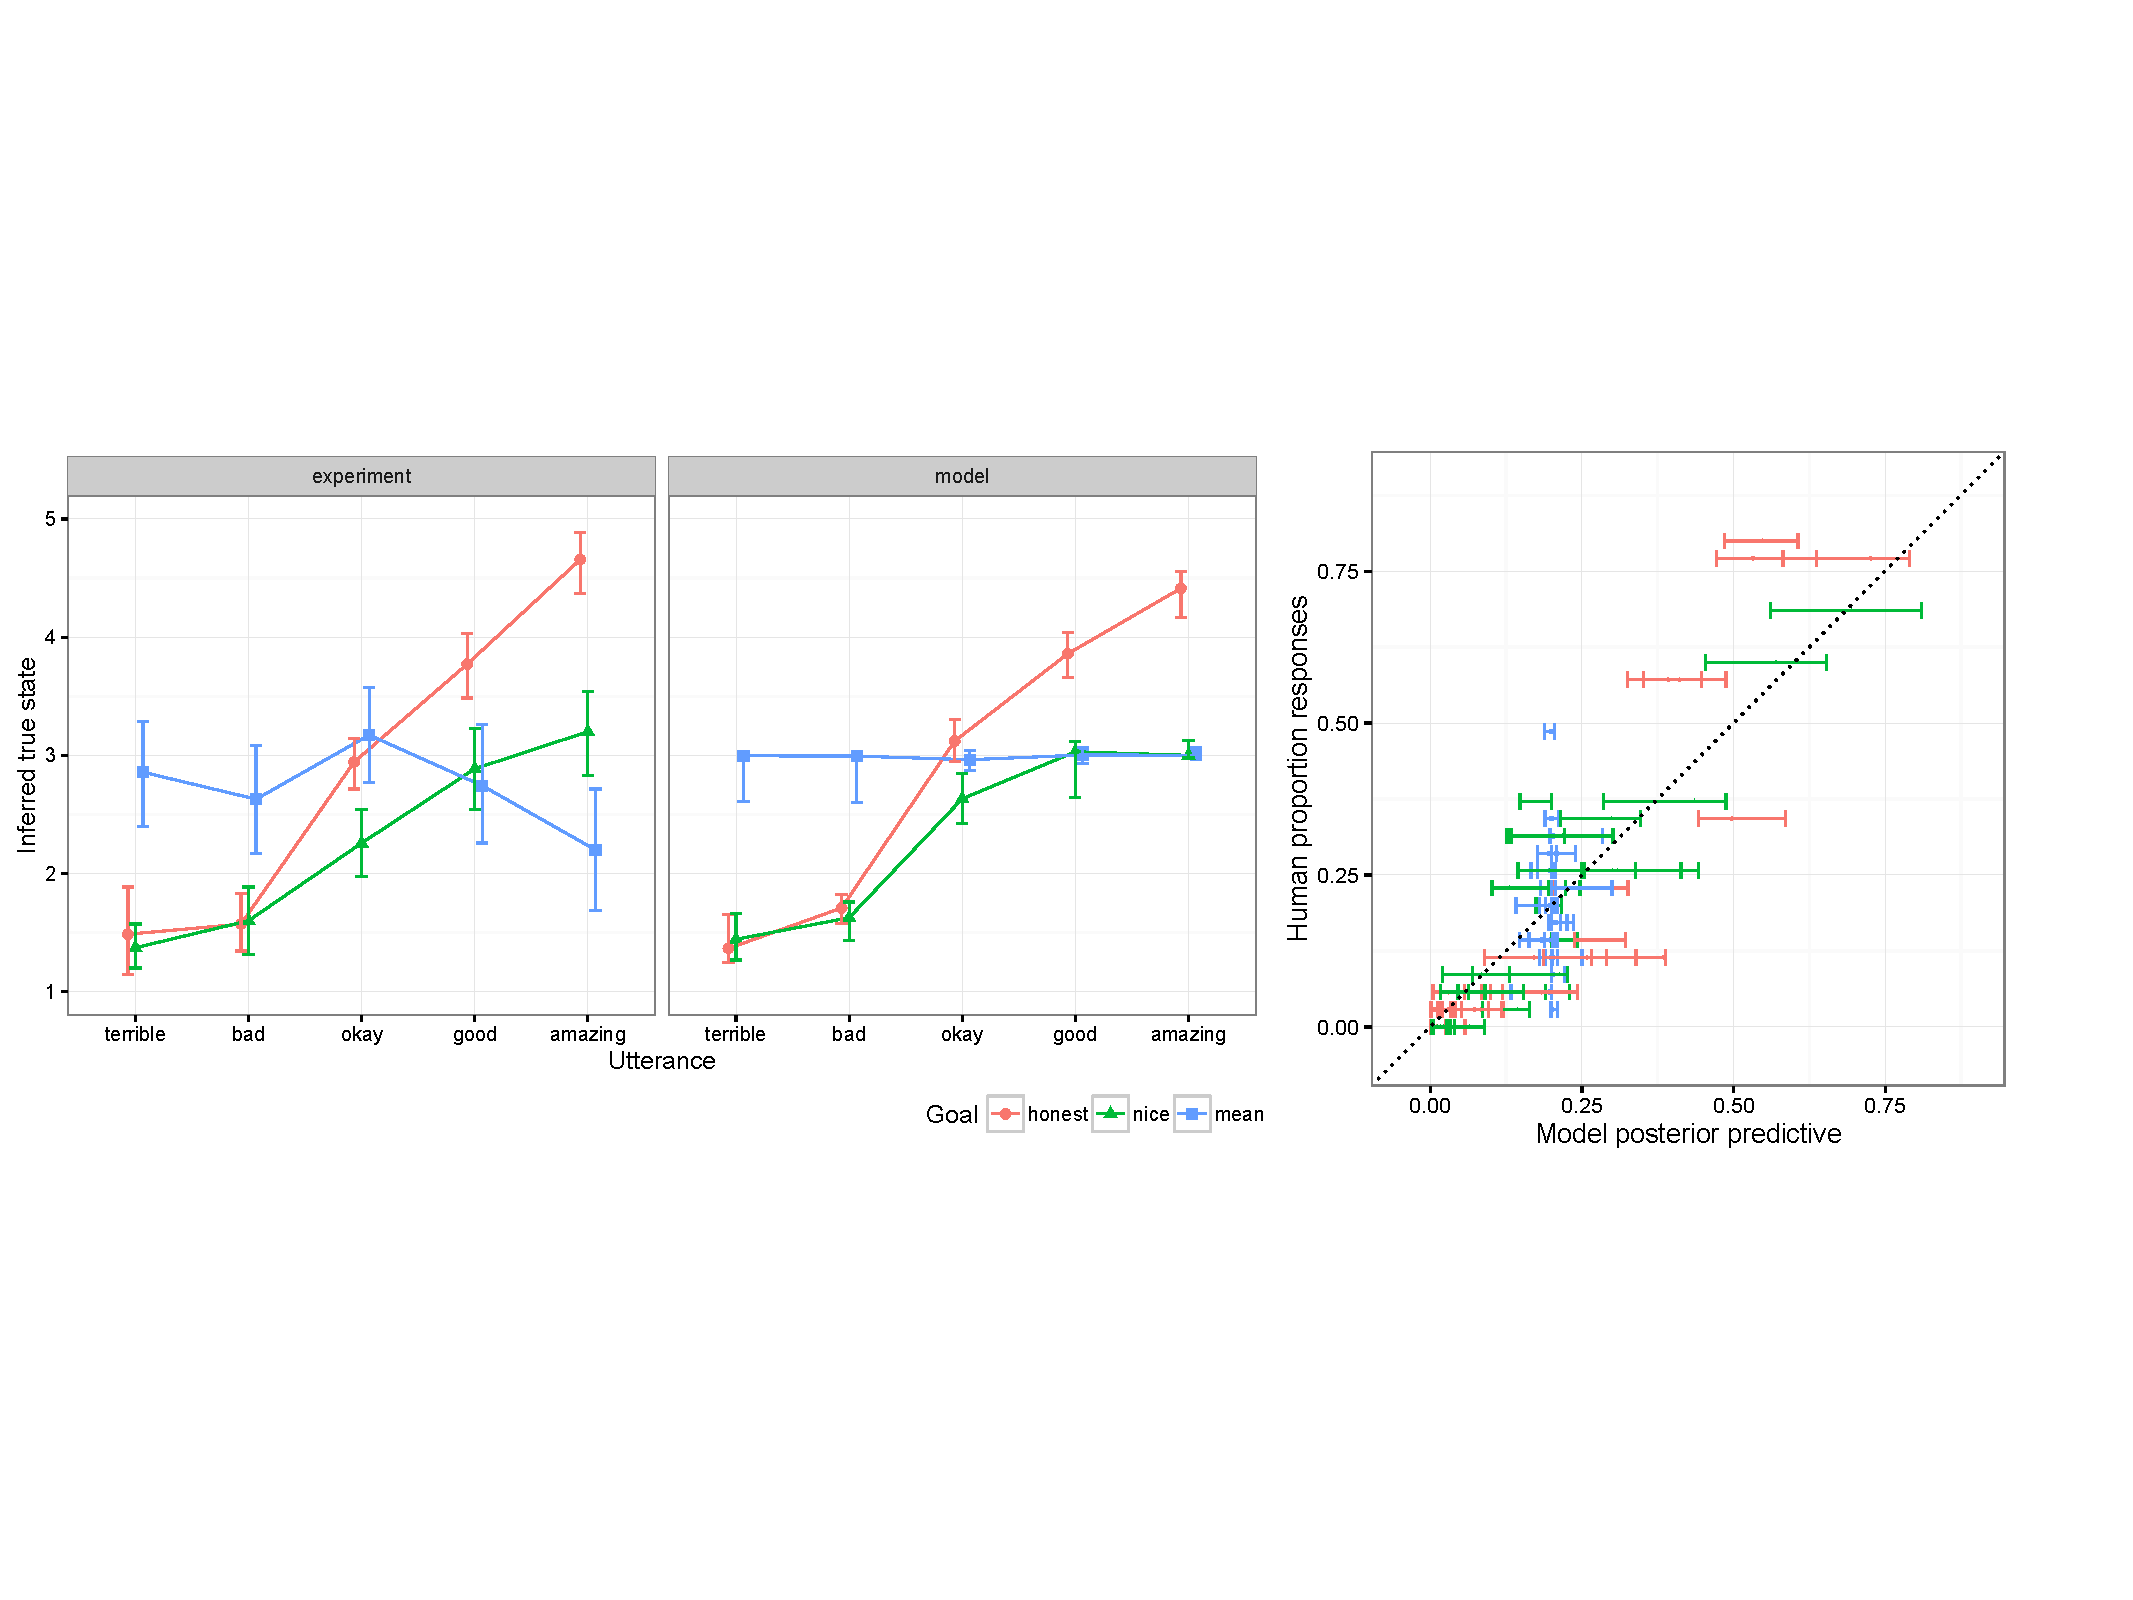
\includegraphics[width=\textwidth]{figures/exp2.pdf}
\caption{\label{fig:expt2} Results from Expt.~2 (left) and model predictions (center) for average states inferred based on a speaker's goal and utterance. Right: Full distribution of human responses vs. model predictions. Error bars represent 95\% confidence intervals for the data and 95\% highest density intervals for the model.}
\end{centering}
\end{figure*}

\subsection{Limitations of previous empirical work}

Our prior work provides a promising start for investigating polite speech phenomena, but there are limitations that narrow the scope of our understanding. First, the empirical support for the model only came from a small, particular population of adults in the US, which, incidentally, is what comprises almost all of major pragmatic language research as well as most experimental work in psychology \citep{henrich2010}. But to examine whether our model or any model of pragmatic language understanding applies universally, it is crucial to examine other groups that are underrepresented in the literature. Specifically, we propose to look at the same inferences in children as well as other cultural groups (e.g. India and South Korea).  

	Second, in our prior work we only considered one particular domain of politeness phenomena: white lies. If other domains of politeness phenomena reflect the same tradeoff between face-saving and informativity, then we should see similar inferential patterns for other kinds of polite speech, such as as indirect remarks (``I wouldn't say that her dress is the most wonderful thing I've ever seen''). Also, we have not looked at what influence the way in which the speakers' communicative goals are determined; one prominent factor is social hierarchy (i.e. ``power distance'' as described by Brown and Levinson), such that subordinates speak more politely to dominant statuses than vice versa. We propose to look at these various kinds of areas and factors associated with polite speech, which will allow us to present a comprehensive theoretical framework to capture the understanding of polite speech.

